\documentclass[pdf,titlepage,a4paper]{report}

\usepackage{graphicx}

%\usepackage{fancyhdr}
%\setlength{\headheight}{15.2pt}
%\pagestyle{fancy}
%\rhead{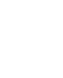
\includegraphics[scale=0.1]{Graphics/BASU_Logo_header.png}}
%\chead{فاز یک پروژه پیشرفته}

\usepackage[hidelinks]{hyperref}

\usepackage[fontsize=18pt]{fontsize}

\usepackage{xepersian}
\settextfont{B Zar}

%\newcommand{\s}{\fontdimen2\font=0.125em}

\begin{titlepage}
	\title{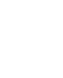
\includegraphics[scale=0.5]{Graphics/BASU_Logo_header.png} \\ \Huge{فاز یک پروژه پیشرفته}}
	\author{متین امیرپناه فر \\ شماره داشنجویی : ۴۰۲۱۲۳۵۸۰۰۳  \and \\ نیما مخملی \\ شماره داشنجویی : ۴۰۲۱۲۳۵۸۰۳۰}
	\date{\today}
\end{titlepage}

\begin{document}
	\maketitle
	\tableofcontents
	
	\begin{abstract}
	\end{abstract}



	\part{کلاس ها}
		
	\newpage
	\section{بازی}
	\paragraph{صفات}
	\subparagraph{رابط گرافیکی}
	\paragraph{متدها}
	\subparagraph{شروع بازی}
	
	
	\newpage
	\section{رابط گرافیکی}
	\paragraph{صفات}
	\paragraph{متدها}
	
	
	\newpage
	\section{زمین بازی}
	\paragraph{صفات}
	\paragraph{متدها}
	
	
	\newpage
	\section{کارت ها}
	\paragraph{صفات}
	\paragraph{متدها}
	
	
	\subsection{کارت های بنفش(ویژه)}
	\paragraph{صفات}
	\subparagraph{}
	
	\paragraph{متدها}
	
	\subsubsection{مترسک}
	\paragraph{صفات}
	\paragraph{متدها}
	
	\subsubsection{طبل زن}
	\paragraph{صفات}
	\paragraph{متدها}
	
	\subsubsection{شاهدخت}
	\paragraph{صفات}
	\paragraph{متدها}
	
	
	\subsection{فصل ها}
	\paragraph{صفات}
	\paragraph{متدها}
	
	\subsubsection{بهار}
	\paragraph{صفات}
	\paragraph{متدها}
	
	\subsubsection{زمستان}
	\paragraph{صفات}
	\paragraph{متدها}
	
	
	\subsection{کارت های زرد(سرباز)}
	\paragraph{صفات}
	\paragraph{متدها}
	\newpage
	
	\section{نشان}
	\paragraph{صفات}
	\paragraph{متدها}
	
	\subsection{نشان بازیکن}
	\paragraph{صفات}
	\paragraph{متدها}
	
	
	\subsection{ایالت}
	\paragraph{صفات}
	\paragraph{متدها}
	
	\section{بازیکن}
	\paragraph{صفات}
	\paragraph{متدها}
	\newpage
	
	
	
	\part{چالش ها}
	\newpage
	
	
	
	\part{پیوندها}
	\section{گیت هاب}
	\href{https://github.com/Matin0789/Condottiere.git}{لینک}
	\newpage
	
	
	
	\part{منابع}
	کتاب برنامه نویسی به زبان سی پلاس پلاس اثر دایتل و دایتل ویرایش دهم
\end{document}
